% ============================================================================
% 5. EXPERIMENTS
% ============================================================================
\section{Experiments}

\subsection{Setup}

We evaluate with \textbf{Gemini~2.5 Flash}~\cite{gemini2024} (closed
frontier), \textbf{DeepSeek-V3}~\cite{deepseekv3} (671B MoE, open-weight),
and \textbf{Qwen2.5-72B}~\cite{qwen25} (72B dense, open-weight),
using greedy decoding ($\tau{=}0$) for deterministic reproducibility.
We report pooled \textbf{Micro-EM} (overall exact match) and
\textbf{Macro-EM} (mean of per-subtype EM, weighting all 13~subtypes
equally).  For list-typed topology tasks (e.g., connected component
membership), we apply \textbf{target-node normalization} (stripping the
queried table from both prediction and gold prior to scoring) ensuring
models are not penalized for harmless self-inclusion.
An \textbf{Oracle} baseline injects gold algorithmic outputs, establishing
an upper bound ($\geq$99.7\% EM across all three models; the residual gap
reflects minor formatting, not reasoning failures).

\subsection{Tier~1: Main Results}

% TABLE 3: Main Results (3 models, with 95% bootstrap CIs)
\begin{table}[t]
\centering
\caption{Tier~1 results (EM~\% $\pm$ 95\% CI, pooled across
5 datasets, 2000 bootstrap resamples).
\textbf{Bold}~=~best non-oracle.}
\label{tab:main-results}
\small
\begin{tabular}{@{}llccccc@{}}
\toprule
Model & & FT & VR & GA & TU & RC \\
\midrule
\multirow{2}{*}{Gem.}
  & Micro & 79.5{\tiny$\pm$2.3} & 73.7{\tiny$\pm$2.7}
  & 77.0{\tiny$\pm$2.5} & \textbf{91.8}{\tiny$\pm$1.7}
  & 83.0{\tiny$\pm$2.3} \\
  & Macro & 83.5{\tiny$\pm$2.6} & 73.9{\tiny$\pm$3.4}
  & 80.3{\tiny$\pm$3.1} & \textbf{91.8}{\tiny$\pm$1.7}
  & 77.6{\tiny$\pm$3.4} \\
\midrule
\multirow{2}{*}{DS}
  & Micro & 70.4{\tiny$\pm$2.8} & 71.6{\tiny$\pm$2.7}
  & 78.4{\tiny$\pm$2.6} & \textbf{91.1}{\tiny$\pm$1.7}
  & 83.1{\tiny$\pm$2.2} \\
  & Macro & 70.1{\tiny$\pm$3.0} & 63.6{\tiny$\pm$3.2}
  & 72.5{\tiny$\pm$3.0} & \textbf{89.8}{\tiny$\pm$2.1}
  & 79.3{\tiny$\pm$2.7} \\
\midrule
\multirow{2}{*}{Qw.}
  & Micro & 63.2{\tiny$\pm$3.0} & 69.5{\tiny$\pm$2.8}
  & 62.8{\tiny$\pm$3.4} & 77.5{\tiny$\pm$3.2}
  & \textbf{82.5}{\tiny$\pm$2.6} \\
  & Macro & 64.8{\tiny$\pm$3.2} & 62.8{\tiny$\pm$3.4}
  & 77.5{\tiny$\pm$3.2} & \textbf{82.5}{\tiny$\pm$2.6}
  & 62.2{\tiny$\pm$3.4} \\
\midrule
\multicolumn{2}{l}{\textit{Oracle}}
  & \multicolumn{5}{c}{99.7 / 99.9 / 100.0} \\
\bottomrule
\end{tabular}
\end{table}

\paragraph{Finding~1: Agentic baselines dominate.}
TU tops Tier~1 at 87--92\% micro-EM, roughly 7--12~pp ahead of the best
static baseline.  RC also clears static methods through code generation.

\paragraph{Finding~2: Triviality Illusion.}
FT looks competitive at 79.5\% micro-EM, but the illusion comes from
\texttt{join\_path} (33\% of questions) inflating the average.
Macro-EM, which weights subtypes equally, puts GA ahead of FT among
static methods; all still trail TU by $>$8~pp (Figure~5, Appendix).

\subsection{Results by Difficulty}

% TABLE 4: By difficulty (3 models)
\begin{table}[t]
\centering
\caption{EM (\%) by difficulty. TU achieves near-perfect easy scores
but plateaus on hard questions alongside static baselines.}
\label{tab:difficulty}
\small
\begin{tabular}{@{}llccccc@{}}
\toprule
Model & Diff. & FT & VR & GA & TU & RC \\
\midrule
\multirow{3}{*}{Gem.}
  & Easy    & 82.7 & 82.5 & 82.2 & \textbf{99.6} & 90.4 \\
  & Med.    & 89.8 & 75.3 & 81.6 & \textbf{99.6} & 91.3 \\
  & Hard    & 56.7 & 47.4 & 56.7 & 59.9 & \textbf{60.9} \\
\midrule
\multirow{3}{*}{DS}
  & Easy    & 82.7 & 84.4 & 87.1 & \textbf{98.0} & 88.8 \\
  & Med.    & 68.3 & 67.3 & 81.3 & \textbf{99.3} & 89.0 \\
  & Hard    & 39.7 & 43.3 & 50.0 & \textbf{60.4} & 58.9 \\
\midrule
\multirow{3}{*}{Qw.}
  & Easy    & 77.4 & 84.0 & 86.6 & \textbf{96.1} & 72.2 \\
  & Med.    & 57.7 & 63.0 & 90.7 & \textbf{72.0} & 64.7 \\
  & Hard    & 33.2 & 40.1 & 51.0 & \textbf{57.0} & 44.1 \\
\midrule
\multicolumn{2}{l}{\textit{Oracle Hard}}
  & \multicolumn{5}{c}{100.0 / 100.0 / 100.0} \\
\bottomrule
\end{tabular}
\end{table}

\paragraph{Easy/Medium inversion.}
Gemini FT scores 89.8\% on Medium but only 82.7\% on Easy.  This occurs
because Medium is dominated by \texttt{join\_path} (342 of 544 Medium
questions), which has high FT accuracy since short FK paths are often
present in the flat schema text.  Easy includes subtypes like
\texttt{count} (number of connected components) that require global
graph access unavailable to FT.  The inversion reflects subtype
composition, not a flaw in difficulty labels.

\begin{figure}[t]
\centering
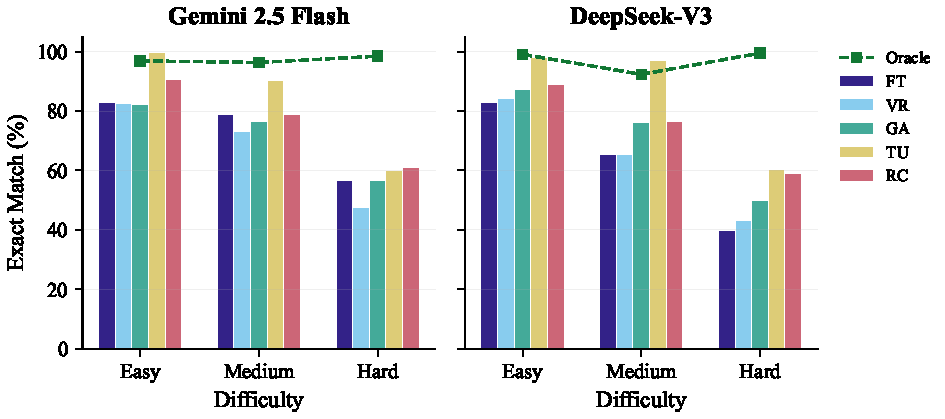
\includegraphics[width=\linewidth]{figures/difficulty_comparison.pdf}
\caption{EM by difficulty level. All baselines plateau on hard
questions while Oracle (dashed) achieves 100\%.}
\label{fig:difficulty}
\end{figure}

\subsection{Per-Subtype Analysis}

\begin{figure*}[t]
\centering
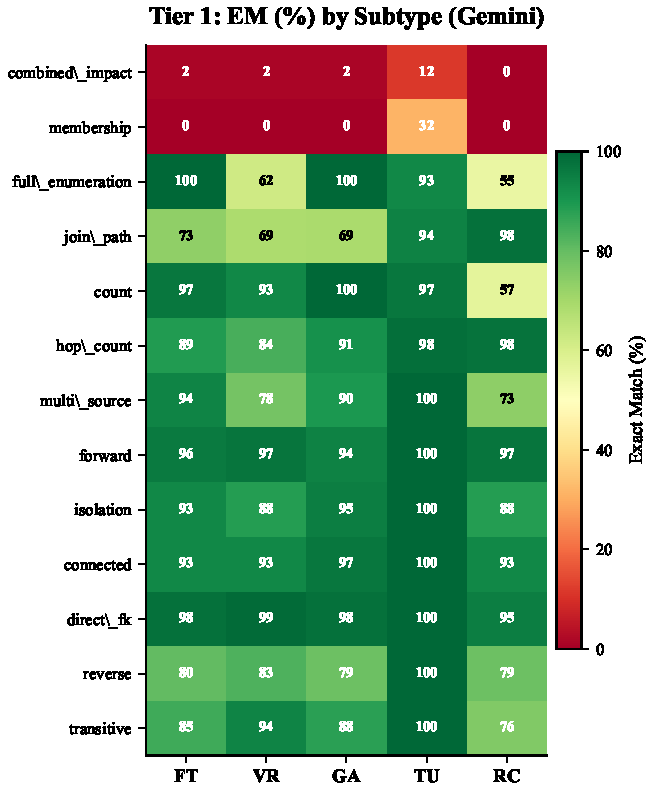
\includegraphics[width=0.85\textwidth]{figures/subtype_heatmap.pdf}
\caption{Tier~1 EM~(\%) by subtype for all three models.  With
target-node normalization, TU and RC now achieve 100\% on
\texttt{membership}, indicating that topology enumeration is fully
solvable with tools.  \texttt{combined\_impact} remains at 0--17\%,
isolating compositional multi-hop reasoning as the core bottleneck.}
\label{fig:heatmap}
\end{figure*}

\paragraph{Finding~3: Hard-task ceiling.}
All baselines plateau at $\sim$60\% on hard questions while Oracle
achieves $>$98\%.  The \texttt{combined\_impact} subtype ($n=69$)
averages only 12\% EM even with TU, identifying compositional
graph reasoning as the fundamental bottleneck.
RC (5~code rounds) shows a similar ceiling to TU (3~tool calls),
suggesting the bottleneck is compositional reasoning itself rather
than interaction budget.

\subsection{Obfuscation}

% TABLE 5 (unchanged data)
\begin{table}[t]
\centering
\caption{Obfuscation penalty (4 datasets). TU is nearly invariant.}
\label{tab:obfuscation}
\small
\begin{tabular}{@{}llccccc@{}}
\toprule
Model & & FT & VR & GA & TU & RC \\
\midrule
\multirow{2}{*}{Gem.}
  & Orig.   & 72.1 & 69.7 & 71.6 & \textbf{91.2} & 87.1 \\
  & $\Delta$ & $-$14.9 & $-$26.0 & $-$27.9 & $-$\textbf{3.4} & $-$7.6 \\
\midrule
\multirow{2}{*}{DS}
  & Orig.   & 68.6 & 74.8 & 82.7 & \textbf{91.4} & 83.4 \\
  & $\Delta$ & $-$27.8 & $-$31.7 & $-$24.3 & $-$\textbf{4.2} & $+$0.6 \\
\bottomrule
\end{tabular}
\end{table}

TU shows minimal degradation ($\Delta{=}{-}3.4$\% Gemini, ${-}4.2$\%
DeepSeek) while static baselines lose 15--32pp.
Obfuscation replaces table names only; column names are preserved,
as all baselines operate on schema-level graph topology where
column semantics play no role.
RC shows near-zero penalty ($\Delta{=}{+}0.6$\% DeepSeek), confirming
that code execution against the graph object is fully invariant to
name perturbation.

\subsection{Tier~2: Value-Level Evaluation}

Tier~2 tests value-level questions requiring interactive row-level data
access (953~questions, 8~subtypes, AdventureWorks + Syn-Logistics).
TU$_{v2}$ achieves 59\% EM (Gemini) and 48\% (DeepSeek) versus 26--31\%
for static baselines.  Both models confirm the same pattern: tools are
\textbf{essential} (\texttt{cascade\_count}: 100\% vs.\ 0\%, both
models) yet \textbf{insufficient} (\texttt{multi\_hop\_trace}: 27\%
both models).  DeepSeek's lower TU score is driven by
\texttt{row\_provenance} (11\% vs.\ 92\%)---it identifies correct
source tables but fails to parse structured row-level tool output.
Full results in Appendix.

\subsection{Discussion}

Our results decompose graph reasoning into \textbf{retrieval-limited}
subtypes (solved by tools) and \textbf{reasoning-limited} subtypes
(unsolved even with tools). The $\sim$35\% of questions that remain
unsolved by both TU and GA largely overlap: their union improves EM by
only 6pp, suggesting the bottleneck is compositional structural reasoning
itself---the capability that GNN encoders are designed to provide.

\begin{figure}[t]
\centering
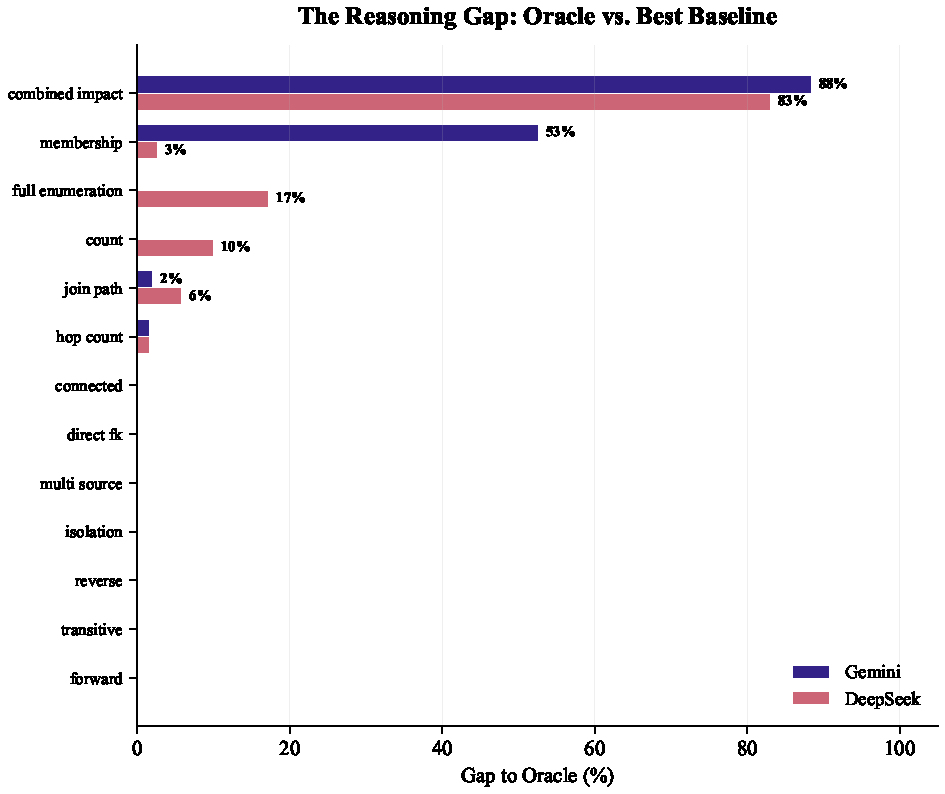
\includegraphics[width=\linewidth]{figures/oracle_gap.pdf}
\caption{Unsolved subtypes: Oracle~EM minus best non-oracle
baseline.  \texttt{combined\_impact} retains$>$83~pp gap;
\texttt{count}, \texttt{full\_enumeration}, and \texttt{transitive}
show 5--25~pp gaps.  The remaining 9 of 13 subtypes are solved
($<$pp).}
\label{fig:oracle-gap}
\end{figure}

\textbf{\texttt{combined\_impact} specification.}
Impact is the union of lineage-downstream tables and their FK-reachable
neighbors: lineage transitive closure then FK BFS.  This two-phase
composition drives the 12\% TU ceiling.
RC receives 5 code-execution rounds (vs.\ TU's 3 tool calls) yet scores
0\% (Gemini) on this subtype, ruling out tool budget
as the primary bottleneck; the failure is compositional planning.

\textbf{GA obfuscation penalty.}
The large GA $\Delta$ ($-$24 to $-$28~pp) reflects two compounding
factors: (1)~loss of semantic priors
(\texttt{DimCustomer}$\to$\texttt{Table\_K}) and (2)~45\% of questions
exceed the 3-hop radius, so obfuscation removes the cues that help LLMs
infer structure beyond the retrieved fragment.

\textbf{Tool tautology.}
TU achieving near-perfect scores on easy subtypes is by design: it
isolates hard failures as genuine reasoning problems.  TU hits 100\% on
\texttt{membership} but still only 12--13\% on
\texttt{combined\_impact}.  The ceiling is not tool availability; it is
compositional multi-step reasoning.

\subsection{Limitations}

We evaluate three frontier LLMs with deterministic single-pass evaluation;
broader model coverage (e.g., reasoning-optimized variants) would
strengthen generality claims.  Tier~2 covers one synthetic and one
real-world dataset; extending to all five schemas is future work.

\paragraph{Responsible use.}
This benchmark is intended for scientific evaluation of LLM capabilities
and limitations.  Researchers should not apply automated agentic tools
or sandboxed code execution to unauthorized or production environments
without appropriate safeguards.

\paragraph{Dataset licenses.}
TPC-DS and TPC-DI are available under the TPC EULA (free for research).
OMOP CDM uses the Apache~2.0 license. AdventureWorks is released under
the Microsoft Public License. Syn-Logistics is our creation, released
under MIT.
